\documentclass{beamer}
\usetheme{CambridgeUS}
\usepackage[utf8]{inputenc}
%\usepackage{default}

%\setbeamertemplate{footline}[frame number]

\setbeamertemplate{headline}
{
    \leavevmode%
    \hbox{%
        \begin{beamercolorbox}[wd=.75\paperwidth,ht=0.001ex,dp=1ex,center]{ }%
            \usebeamerfont{ } 
        \end{beamercolorbox}%
        \begin{beamercolorbox}[wd=.28\paperwidth,ht=0.001ex,dp=1ex,right]{ }%
            \usebeamerfont{ }\hspace*{2em}
             / \hspace*{2ex}
        \end{beamercolorbox}}%
        \vskip0pt%
    }

\setbeamertemplate{footline}
{
    \leavevmode%
    \hbox{%
        \begin{beamercolorbox}[wd=.28\paperwidth,ht=2.25ex,dp=1ex,center]{author in head/foot}%
            \usebeamerfont{author in head/foot}\insertshortauthor{}
        \end{beamercolorbox}%
        \begin{beamercolorbox}[wd=.28\paperwidth,ht=2.25ex,dp=1ex,right]{date in head/foot}%
            \usebeamerfont{date in head/foot}\insertshortdate{}\hspace*{2em}
            \insertframenumber{} / \inserttotalframenumber\hspace*{2ex} 
        \end{beamercolorbox}}%
        \vskip0pt%
    }

\author{Unai Aseguinolaza Aguirreche}
\title{Anharmonic effects in thermoelectric and 2D materials}
\institute{Supervided by Aitor Bergara and Ion Errea}
\date{\today}
\titlegraphic{
\includegraphics[width=.35\textwidth,height=.25\textheight]{Pictures/LOGOS/EHU.jpg}
              
\includegraphics[width=.25\textwidth,height=.3\textheight]{Pictures/LOGOS/CFM.jpg}
              
\includegraphics[width=.35\textwidth,height=.2\textheight]{Pictures/LOGOS/DIPC.jpg}}

\begin{document}

\setbeamertemplate{navigation symbols}{}

\begin{frame}
 \titlepage
\end{frame}

\begin{frame}

\frametitle{General outline}
\begin{enumerate}
	\item Thermoelectric monochalcogenides (part 1)
	\begin{itemize}
		\item Bulk SnSe and SnS
		\item Monolayer SnSe
	\end{itemize}
	\vspace{2cm}
\item 2D materials (part 2)
	\begin{itemize}
		\item Graphene
	\end{itemize}
\end{enumerate}

\end{frame}

\begin{frame}

\frametitle{Outline}
\begin{itemize}
\item Introduction
\vspace{0.5cm}
\item Theoretical framework
\vspace{0.5cm}
\item Part 1: Thermoelectric monochalcogenides
\vspace{0.5cm}
\item Part 2: 2D materials
\vspace{0.5cm}
\item Conclusions
\end{itemize}

\end{frame}

\begin{frame}

\frametitle{Introduction}
\vspace{-0.5cm}
\begin{equation}
ZT=\frac{S^{2}\sigma T}{\kappa}, \hspace{0.6cm} S=-\frac{\Delta V}{\Delta T}%, \hspace{0.6cm} ZT_{ave}=\frac{1}{T_{h}-T_{c}}\int_{T_{c}}^{T_{c}}ZTdT
\nonumber
\end{equation}
\begin{center}
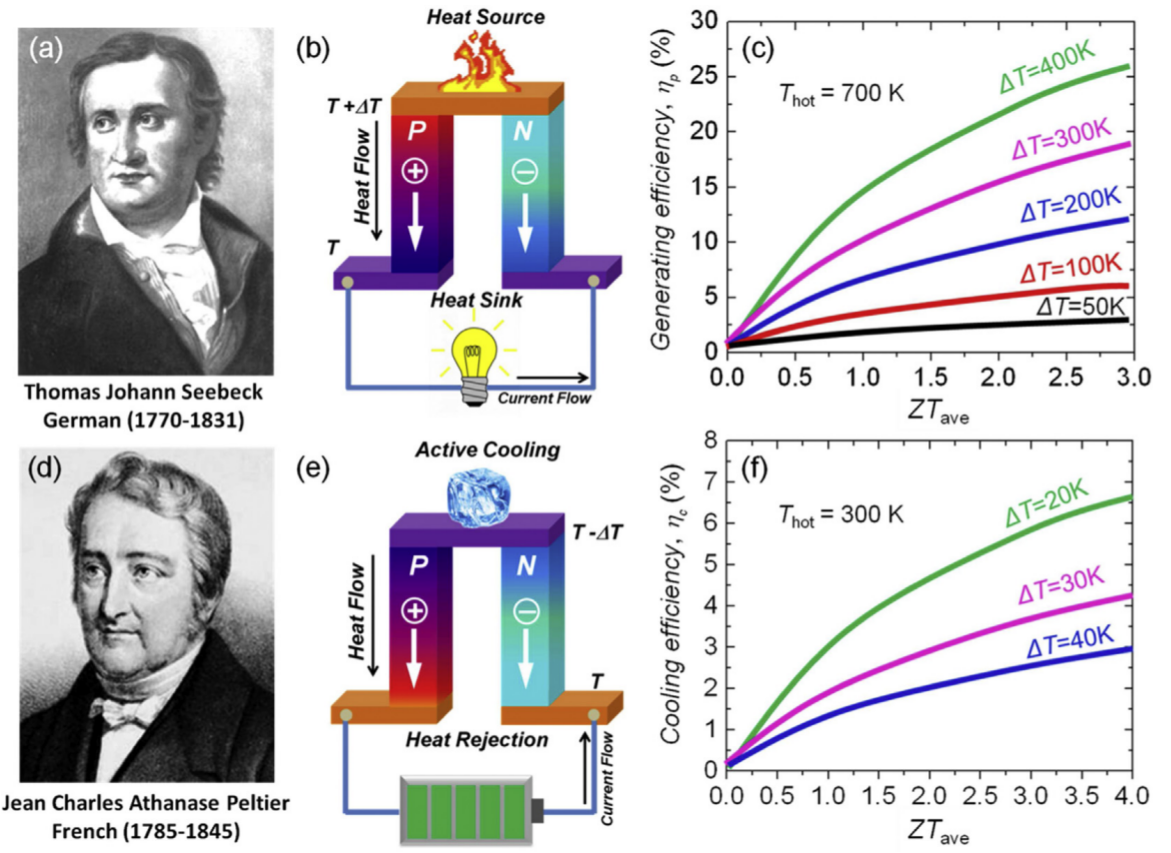
\includegraphics[width=0.7\linewidth]{Pictures/INTRO/generation-cooling.png}
\end{center}
\vspace{-0.1cm}
\begin{tiny}
X. Zhang, L-D. Zhao / Journal of Materiomics 1 (2015) 92-105
\end{tiny}

\end{frame}

\begin{frame}

\frametitle{Introduction}
\vspace{-0.5cm}
\begin{center}
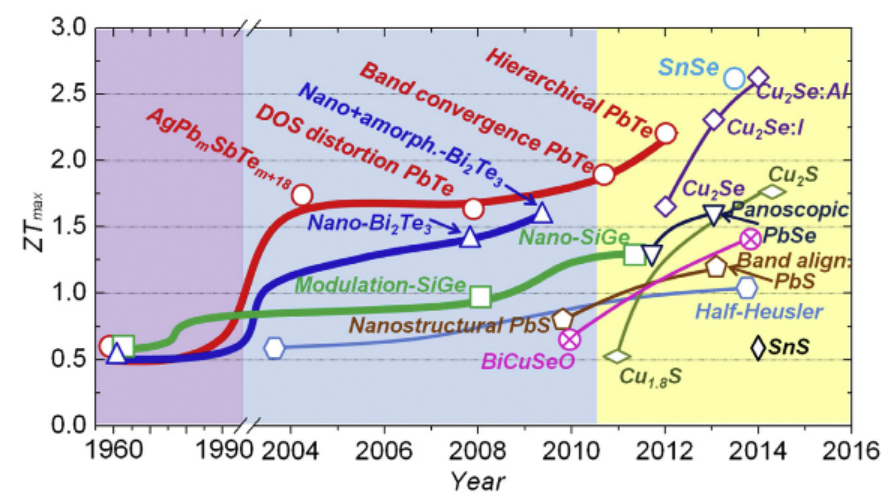
\includegraphics[width=0.7\linewidth]{Pictures/INTRO/ztvstemp.png}
\end{center}
\vspace{-0.1cm}
\begin{itemize}
\item $ZT_{max}$ low and in narrow temperature ranges
\item Very limited technological applications.
\end{itemize}
\begin{tiny}
X. Zhang, L-D. Zhao / Journal of Materiomics 1 (2015) 92-105
\end{tiny}

\end{frame}

\begin{frame}

\frametitle{Introduction}
\vspace{-0.5cm}
\begin{center}
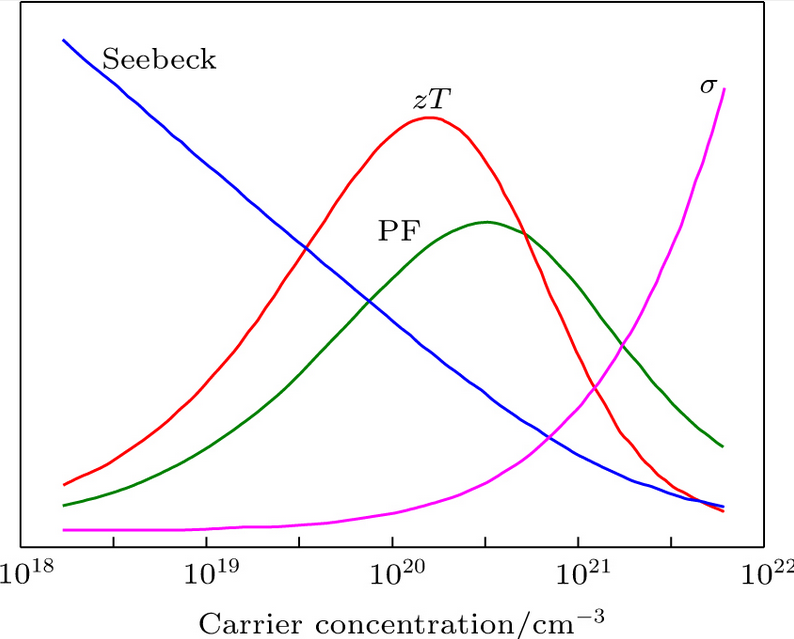
\includegraphics[width=0.5\linewidth]{Pictures/INTRO/decoupling.png}
\end{center}
\vspace{-0.1cm}
\begin{itemize}
\item The physical magnitudes that define $ZT$ are correlated
\item How to overcome:
	\begin{itemize}
	\item Doping + nanostructuring
	\item Proximity to phase transitions
	\item \dots
	\end{itemize}
\end{itemize}

\end{frame}

\begin{frame}

\frametitle{Introduction}
\vspace{-0.5cm}
\begin{center}
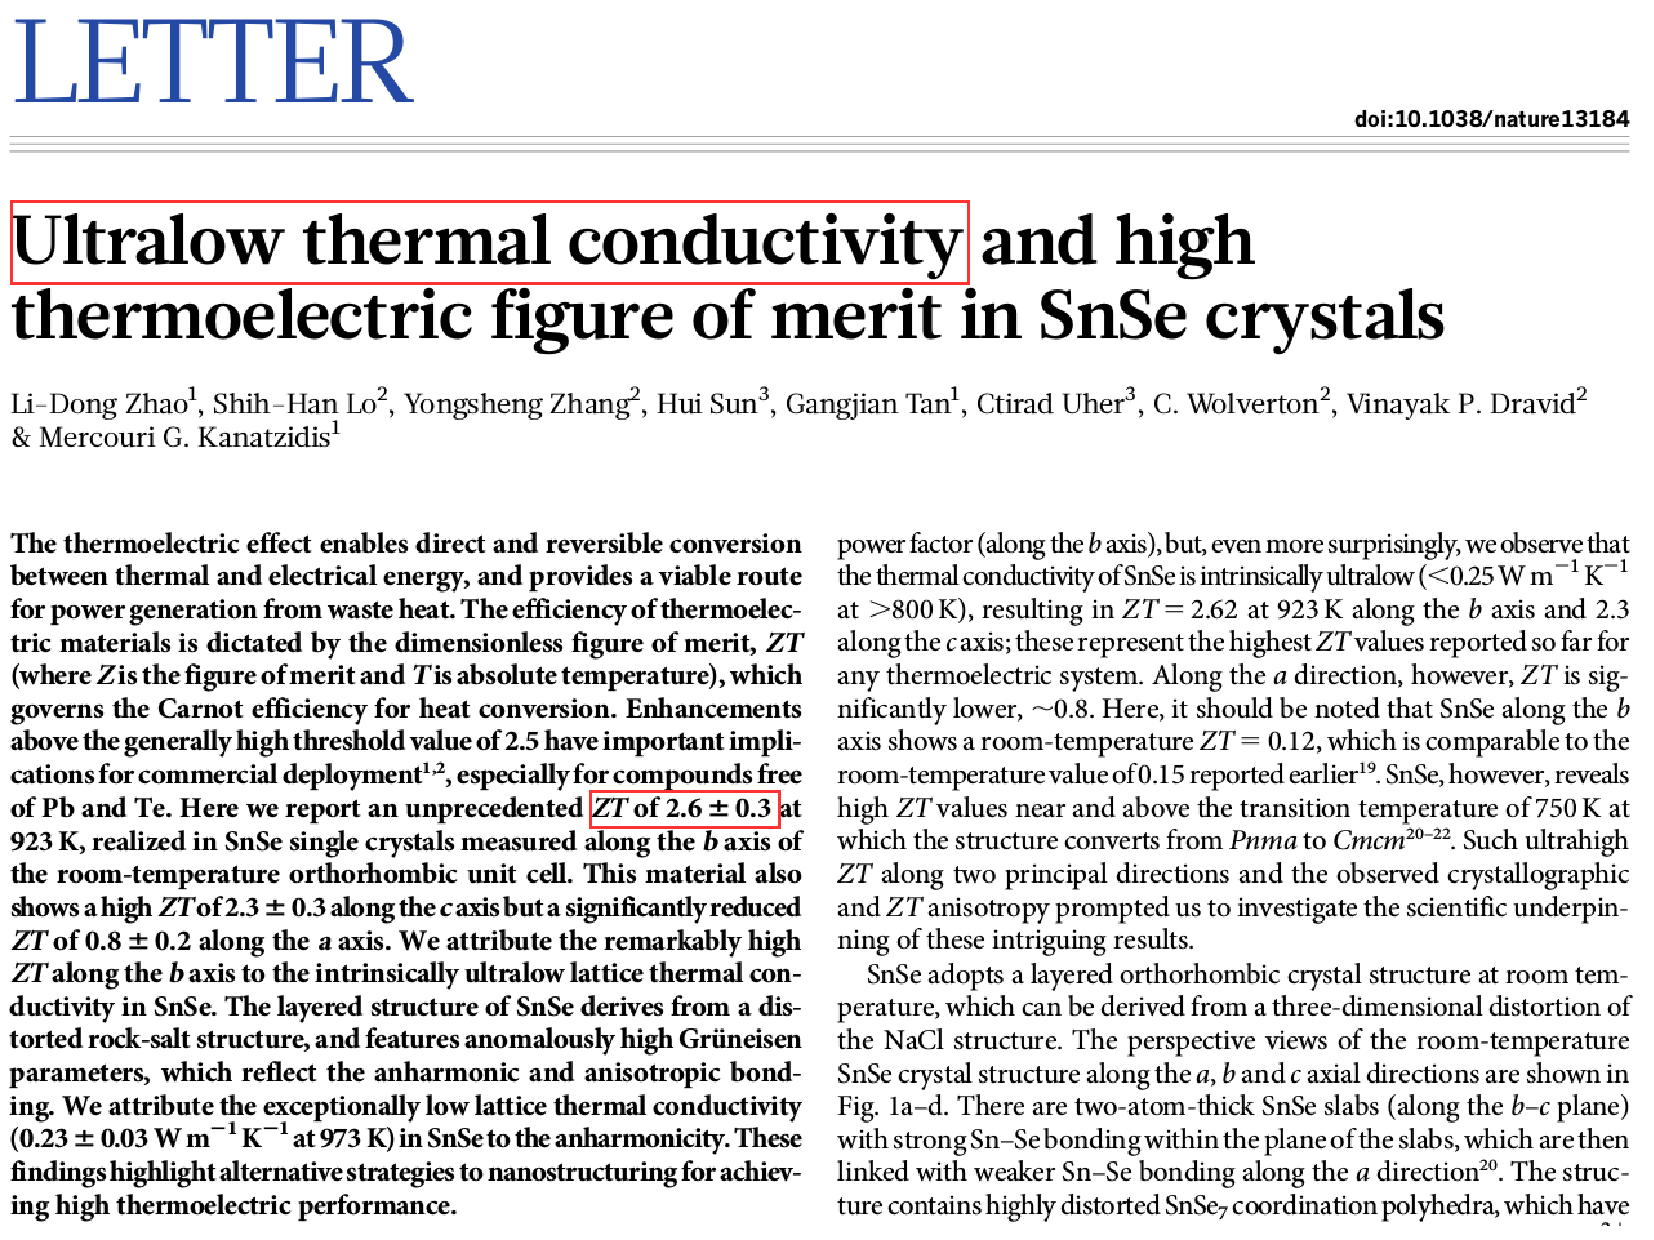
\includegraphics[width=0.7\linewidth]{Pictures/INTRO/natureSnSe.pdf}
\end{center}
\begin{itemize}
\item The best thermoelectric material so far: Intrinsic semiconductor with low lattice thermal 
conductivity ($\kappa=\kappa_{el} + \kappa_{l}$) 
\end{itemize}

\end{frame}

\begin{frame}

\frametitle{Introduction}
\vspace{-0.5cm}
\begin{center}
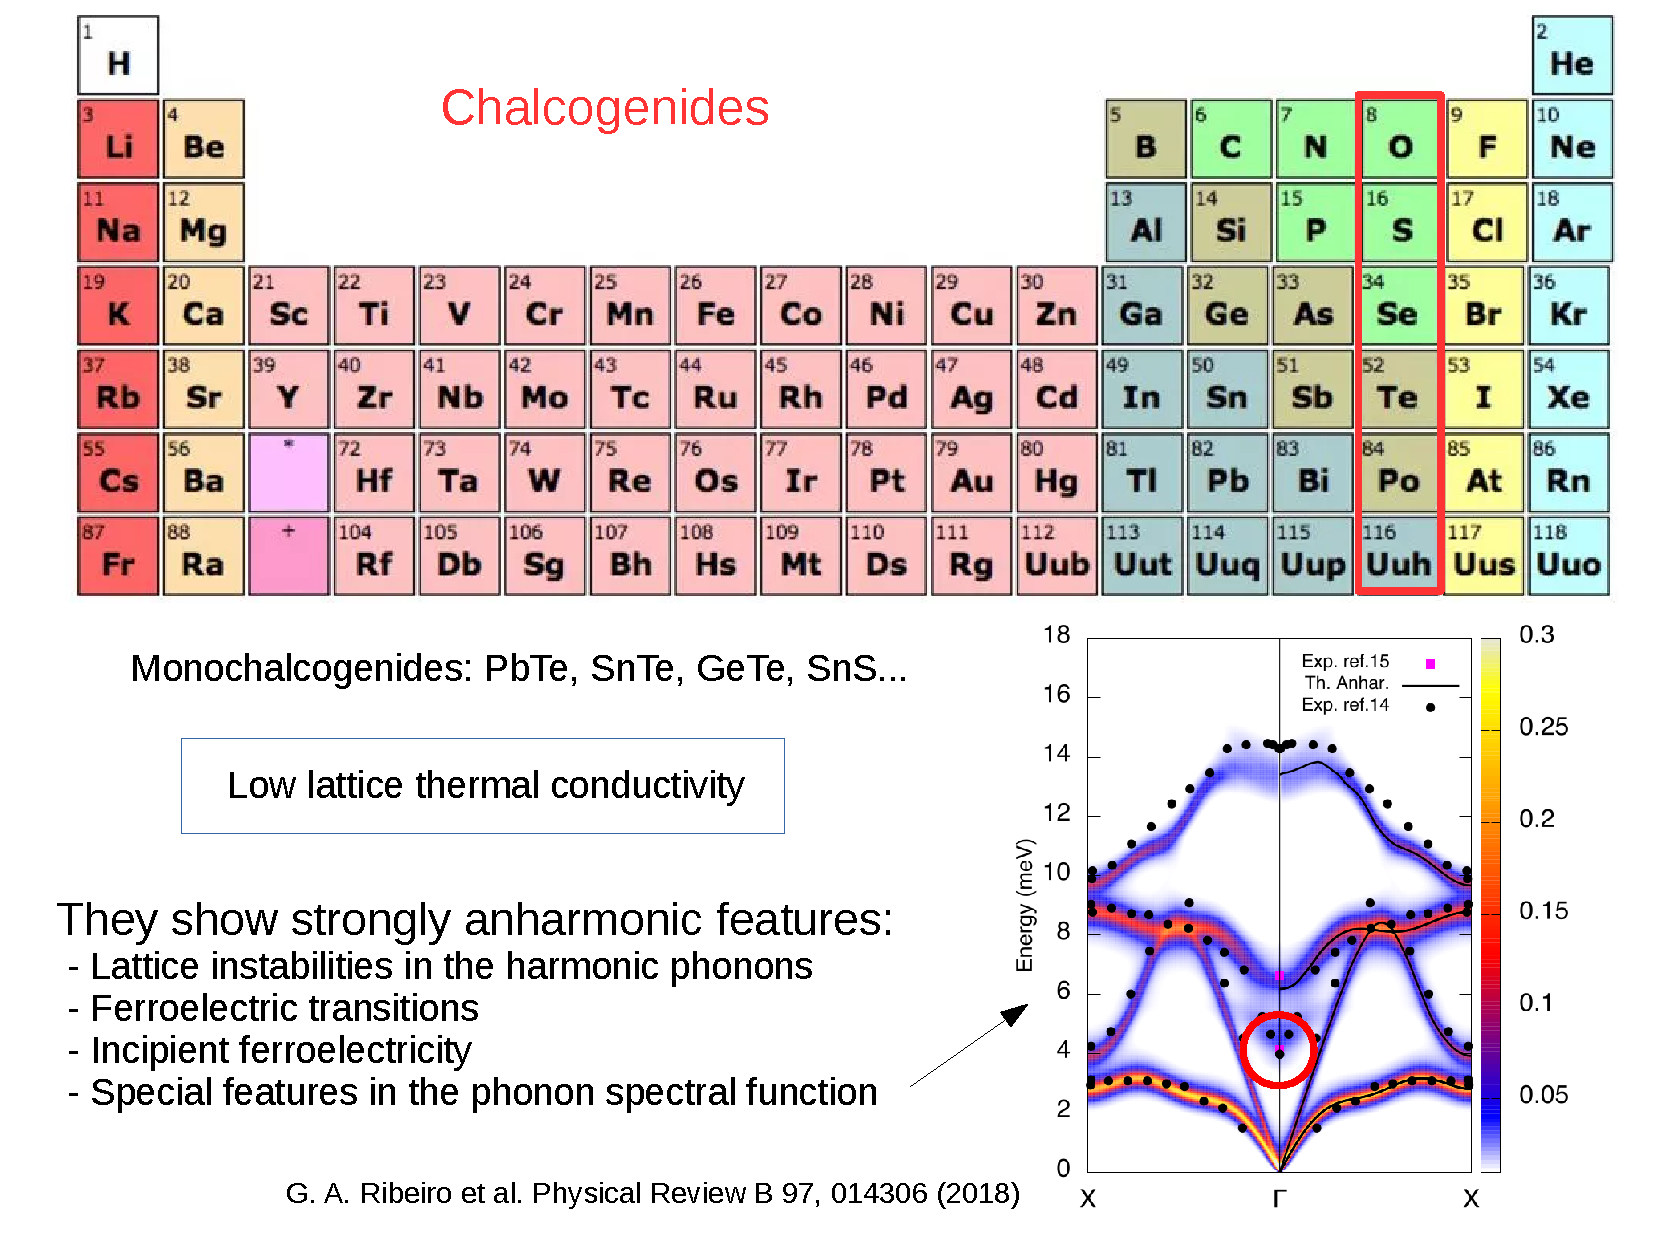
\includegraphics[width=0.85\linewidth]{Pictures/INTRO/chalcogenides.pdf}
\end{center}

\end{frame}

\begin{frame}

\frametitle{Introduction}
\vspace{-0.5cm}
\begin{center}
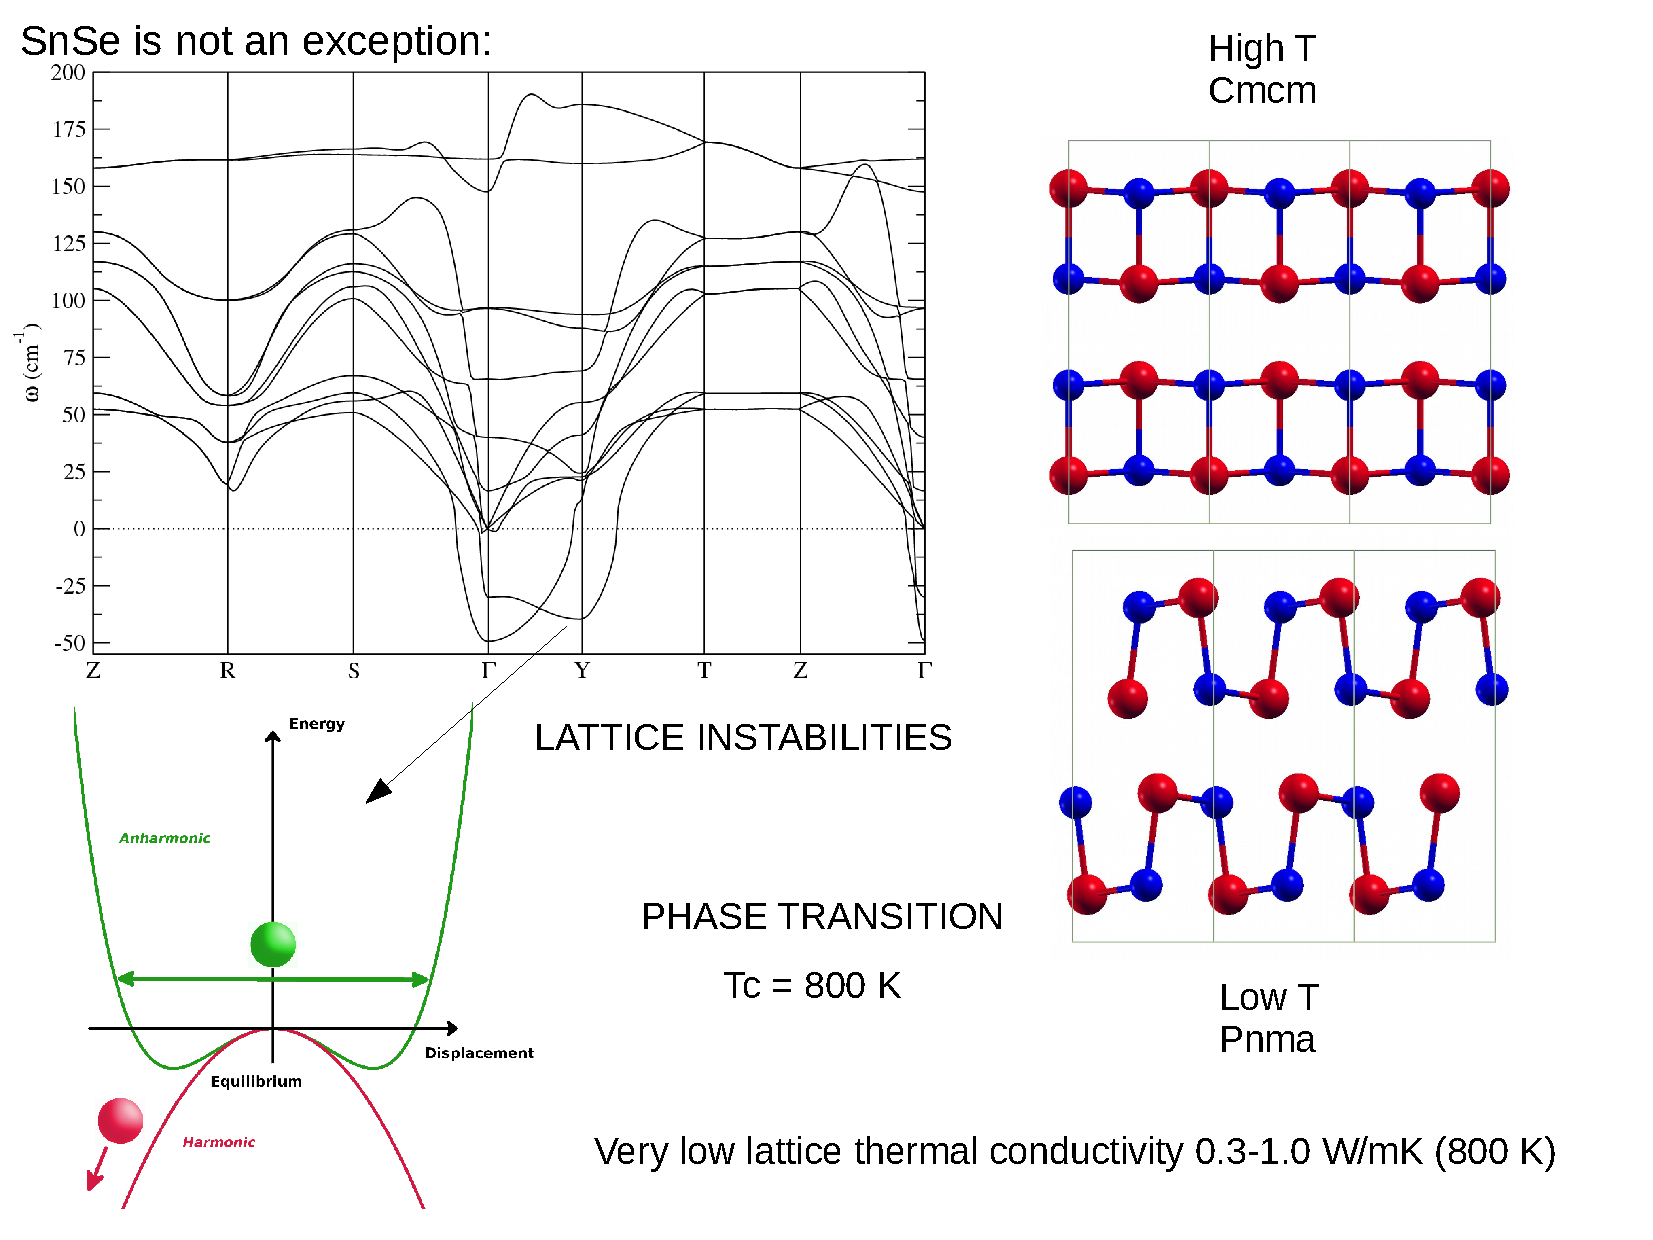
\includegraphics[width=0.85\linewidth]{Pictures/INTRO/SnSeIntro.pdf}
\end{center}

\end{frame}

\end{document}
